\documentclass[a4paper,12pt]{article}

\title{Biology 30 IB \\ Nervous System}
\author{Jad Chehimi}

% document setup
\renewcommand{\familydefault}{\sfdefault}
\linespread{1.25}
\usepackage[margin=1in]{geometry}
\usepackage{setspace}
\usepackage{enumitem}
\setlist{nosep}
\usepackage{color,soul}
\setcounter{secnumdepth}{0}

% tools
\usepackage[hidelinks]{hyperref}
\usepackage{float}
%% images
\usepackage{graphicx}
\graphicspath{ {./images/} }
%% science
\usepackage{siunitx}
%% chemistry
%\usepackage[version=4]{mhchem}

\begin{document}
\maketitle

% temp
\begin{center}
\Huge
Unfinished!
\normalsize
\end{center}
% temp

\tableofcontents

\pagebreak

\section{(13.1) The Nervous System}
\begin{itemize}
    \item{\textbf{Equilibrium/Homeostasis} = balance, main job of nervous system is to maintain this}
    \item{
            Nervous system contains...
            \begin{itemize}
                \item{Brain}
                \item{Spinal cord}
                \item{Nerves}
            \end{itemize}
        }
\end{itemize}

\section{Divisions of the Nervous System}
\begin{figure}[H]
    \centering
    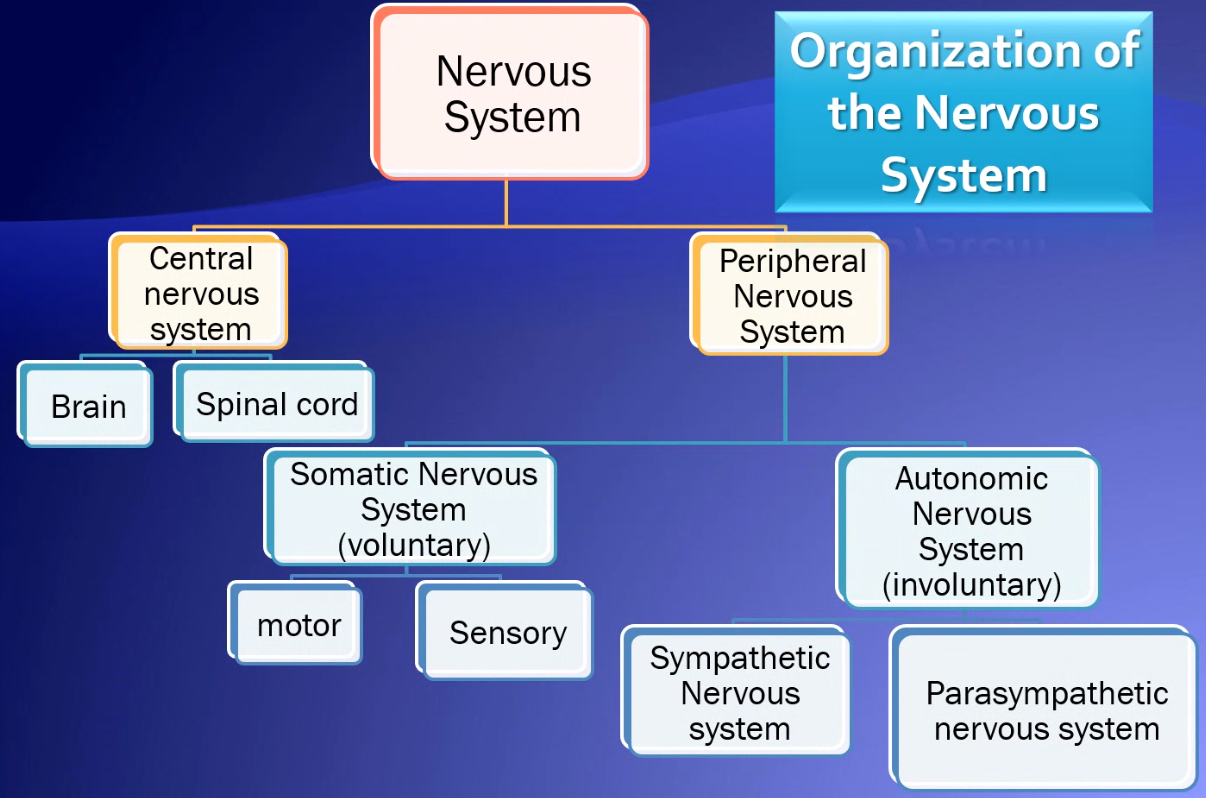
\includegraphics[width=\textwidth]{flowchart}
\end{figure}

\subsection{Central Nervous System (CNS)}
\begin{itemize}
    \item{Integrates and processes information}
    \item{Consists of \hl{brain} and \hl{spinal cord}}
\end{itemize}

\subsection{Peripheral Nervous System (PNS)}
\begin{itemize}
    \item{\hl{Messenger nerves}; bring \hl{info to and from} the central nervous system}
    \item{
            Consists of nerves that...
            \begin{itemize}
                \item{carry sensory messages to the CNS}
                \item{send info from the CNS to the muscles and glands}
            \end{itemize}
        }
\end{itemize}

\subsubsection{Somatic Nervous System (SNS)}
\begin{itemize}
    \item{Voluntary control}
    \item{
            Includes neurons for...
            \begin{itemize}
                \item{\hl{Voluntary motor/muscle control} = carry signals from the CNS to the skeletal muscles}
                \item{\hl{Sensory receptors} = carry sensory info to the CNS}
            \end{itemize}
        }
\end{itemize}

\subsection{Autonomic Nervous System (ANS)}
\begin{itemize}
    \item{Divisions of automatic nerves that are \hl{antagonistic/oppose each other}}
    \item{Regulates involuntary control processes (automatic) such as breathing or heartbeat}
    \item{
            Controls...
            \begin{itemize}
                \item{glandular secretions}
                \item{function of \hl{smooth and cardiac muscles}}
            \end{itemize}
        }
\end{itemize}
\subsubsection{Sympathetic Nervous System}
\begin{itemize}
    \item{"Fight or flight (or freeze)" responses}
    \item{\hl{Prioritizes urgent} functions, such as by speeding up rates of breathing, heart rate, etc.}
    \item{\hl{Disables non-urgent} functions, such as digesting}
\end{itemize}

\subsubsection{Parasympathetic Nervous System}
\begin{itemize}
    \item{"Rest and digest" responses}
    \item{\hl{Restores normal priorities} restored, slows down rates of breathing, heart rate, etc.}
    \item{\hl{Re-enables non-urgent} functions, such as digesting}
\end{itemize}

\section{Cells of the Nervous System}
\begin{itemize}
    \item{
            \textbf{Neurons} = functional units of nervous system, \hl{tissues of neurons} are called \textbf{nerves}
            \begin{itemize}
                \item{\hl{Respond} to physical and chemical stimuli}
                \item{\hl{Conduct} electrochemical signals}
                \item{\hl{Release} chemicals that regulate various body processes}
            \end{itemize}
        }
    \item{
            \textbf{Glial Cells} = supporting cells of nerve cells
            \begin{itemize}
                \item{Nourish neurons, remove wastes, \& defend against infection}
                \item{Provide a supporting framework for all nervous-system tissue}
            \end{itemize}
        }
\end{itemize}


\end{document}
